\documentclass[11pt,a4paper]{article}
\usepackage[utf8]{inputenc}
\usepackage[T1]{fontenc}
\usepackage{amsfonts}
\usepackage[french]{babel}
\frenchbsetup{StandardLists=true}
\usepackage{enumitem}
\usepackage{amssymb}
\usepackage{amsmath}
\DeclareMathOperator{\e}{e}

\usepackage[left=2cm,right=2cm,top=2cm,bottom=2cm]{geometry}
\usepackage{multirow}
\usepackage[dvipsnames]{xcolor}
\usepackage{parskip}
\usepackage{caption}
\usepackage{fouriernc}
\usepackage{graphicx}
\usepackage{setspace}
\singlespacing

\usepackage{tcolorbox}
\usepackage{framed}
\usepackage{multicol}
\usepackage{fancybox}
\usepackage{fancyhdr}
\pagestyle{fancy}
\renewcommand\headrulewidth{1pt}
\fancyhead[L]{Lycée Denis Diderot }
\fancyhead[R]{Classe de Première Bac Pro}
\setcounter{page}{3}\fancyfoot[C]{page \thepage}
\fancyfoot[R]{Année 2025-2026}
\fancyfoot[L]{Alexis RUIZ}
\usepackage{pstricks,pst-plot}
\usepackage{tikz}
\usepackage{tkz-tab}
\usetikzlibrary{arrows}
\usepackage{pifont}
\usepackage{wrapfig}
\usepackage{pgfplots,mathtools}
\usepackage[tikz]{bclogo}

\newtcolorbox{mybox}{colback=blue!10!white,colframe=black!5!black}
\newtcolorbox{mybox1}{colback=white,colframe=black!5!black}

\newcommand{\cadre}[1]{%
\vspace{2mm}
\begin{bclogo}[couleur=white,logo=,arrondi=0.3,barre=none]{%
\rule{0mm}{#1mm}}\par
\medskip
\end{bclogo}}

% Commande pour le texte rouge
\newcommand{\rouge}[1]{\textcolor{red}{#1}}

\begin{document}

\begin{mybox1}
NOM : \hfill Prénom : \hfill ~~
\end{mybox1}

\vfill
\begin{mybox}
\begin{center}
\textbf{\Large Contrôle 1 - Mesures du courant (CORRIGÉ)}
\end{center}
\end{mybox}

\vfill 

\begin{mybox1}
Exercice 1 : Convertir (avec 1A = 1000 mA) ~ \hfill ~~ 1,5 pts
\end{mybox1}

\vspace{3mm}

\begin{multicols}{3}
$1200$mA = \rouge{1,2} A 
\vspace{5mm}

$800$mA = \rouge{0,8} A 
\vspace{5mm}

$21380$mA = \rouge{21,38} A 
\vspace{5mm}

$1,01$A = \rouge{1010} mA
\vspace{5mm}

$10,81$A = \rouge{10810} mA
\vspace{5mm}

$0,801$A = \rouge{801} mA
\vspace{5mm}
\end{multicols}

\begin{mybox1}
Exercice 2 : Application de la loi des noeuds ~ \hfill ~~ 3,5 pts
\end{mybox1}

\begin{enumerate}
\item Indiquer à l'aide de flèches le sens du courant dans chaque branche.
\begin{center}
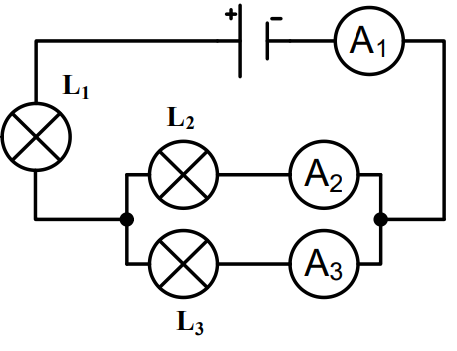
\includegraphics[scale=0.4]{images/exercice 3.png}
\end{center}

\item Soit $\mathrm{I_1 }$
l’intensité du courant dans la branche principale, $\mathrm{I_2 }$ dans la branche de $\mathrm{L_2}$ et $\mathrm{I_3 }$ dans la branche de $\mathrm{L_3}$. \\[5mm]
Écrire la loi des noeuds.~~\rouge{$\mathrm{I_1 = I_2 + I_3}$} 

\item On donne $\mathrm{I_2 }$ = 1,45 A et $\mathrm{I_3 }$ = 550 mA. Calculer $\mathrm{I_1 }$ \\

\rouge{$\mathrm{I_1 = 1,45 + 0,55 = 2,00\ A}$}

\item La lampe $\mathrm{L_3 }$ grille. L'ampèremètre $\mathrm{A_2 }$ mesure alors $\mathrm{I_2 }$ = 2 A. 
Que mesurera l'ampèremètre $\mathrm{A_3 }$ ? \\

\rouge{$\mathrm{I_3 = 0\ A}$ (lampe grillée)}

\item Que mesurera l'ampèremètre $\mathrm{A_1 }$ si la lampe $\mathrm{L_3}$ est toujours grillée ? \\

\rouge{$\mathrm{I_1 = I_2 + I_3 = 2 + 0 = 2\ A}$}
\end{enumerate}

\vfill 
\begin{mybox}
ENIGME BONUS (+1)
\end{mybox}

Voici une suite logique de nombres : 6 ; 4 ; 8 ; 5 ; 15 …  
\cadre{10}


\vfill

\end{document}
